% Copyright (c) 2014,2016 Casper Ti. Vector
% Public domain.

\chapter{区块链的实名交易监督系统設計}
%\pkuthssffaq % 中文测试文字。
本論文提出区块链的实名交易监督系统(Blockchain Real-name Transaction Monitoring System,BRTMS),以下簡稱BRTMS,BRTMS以密碼貨幣比特幣實作,BRTMS包含三個子系統,商店和商品信息管理子系統(Store and Merchandise Information Management Sub-System,SMIMSS)、商家移動裝置收款及交易子系統(Store Mobile payment Collection and Transaction、Sub-System,SMCTSS)、客戶端移動支付和交易子系統(Client Mobile Payment and Transaction Sub-System,CMPTSS),我們將在稍後描述這些子系統。

	\section{BRTMS數據庫設計}

		\subsection{原數據庫}
		区块链的实名交易监督系统應用了四個原數據庫,分別為使用者數據庫、產品數據庫、商家數據庫、交易數據庫:

		\begin{figure}[h]
			\centering
			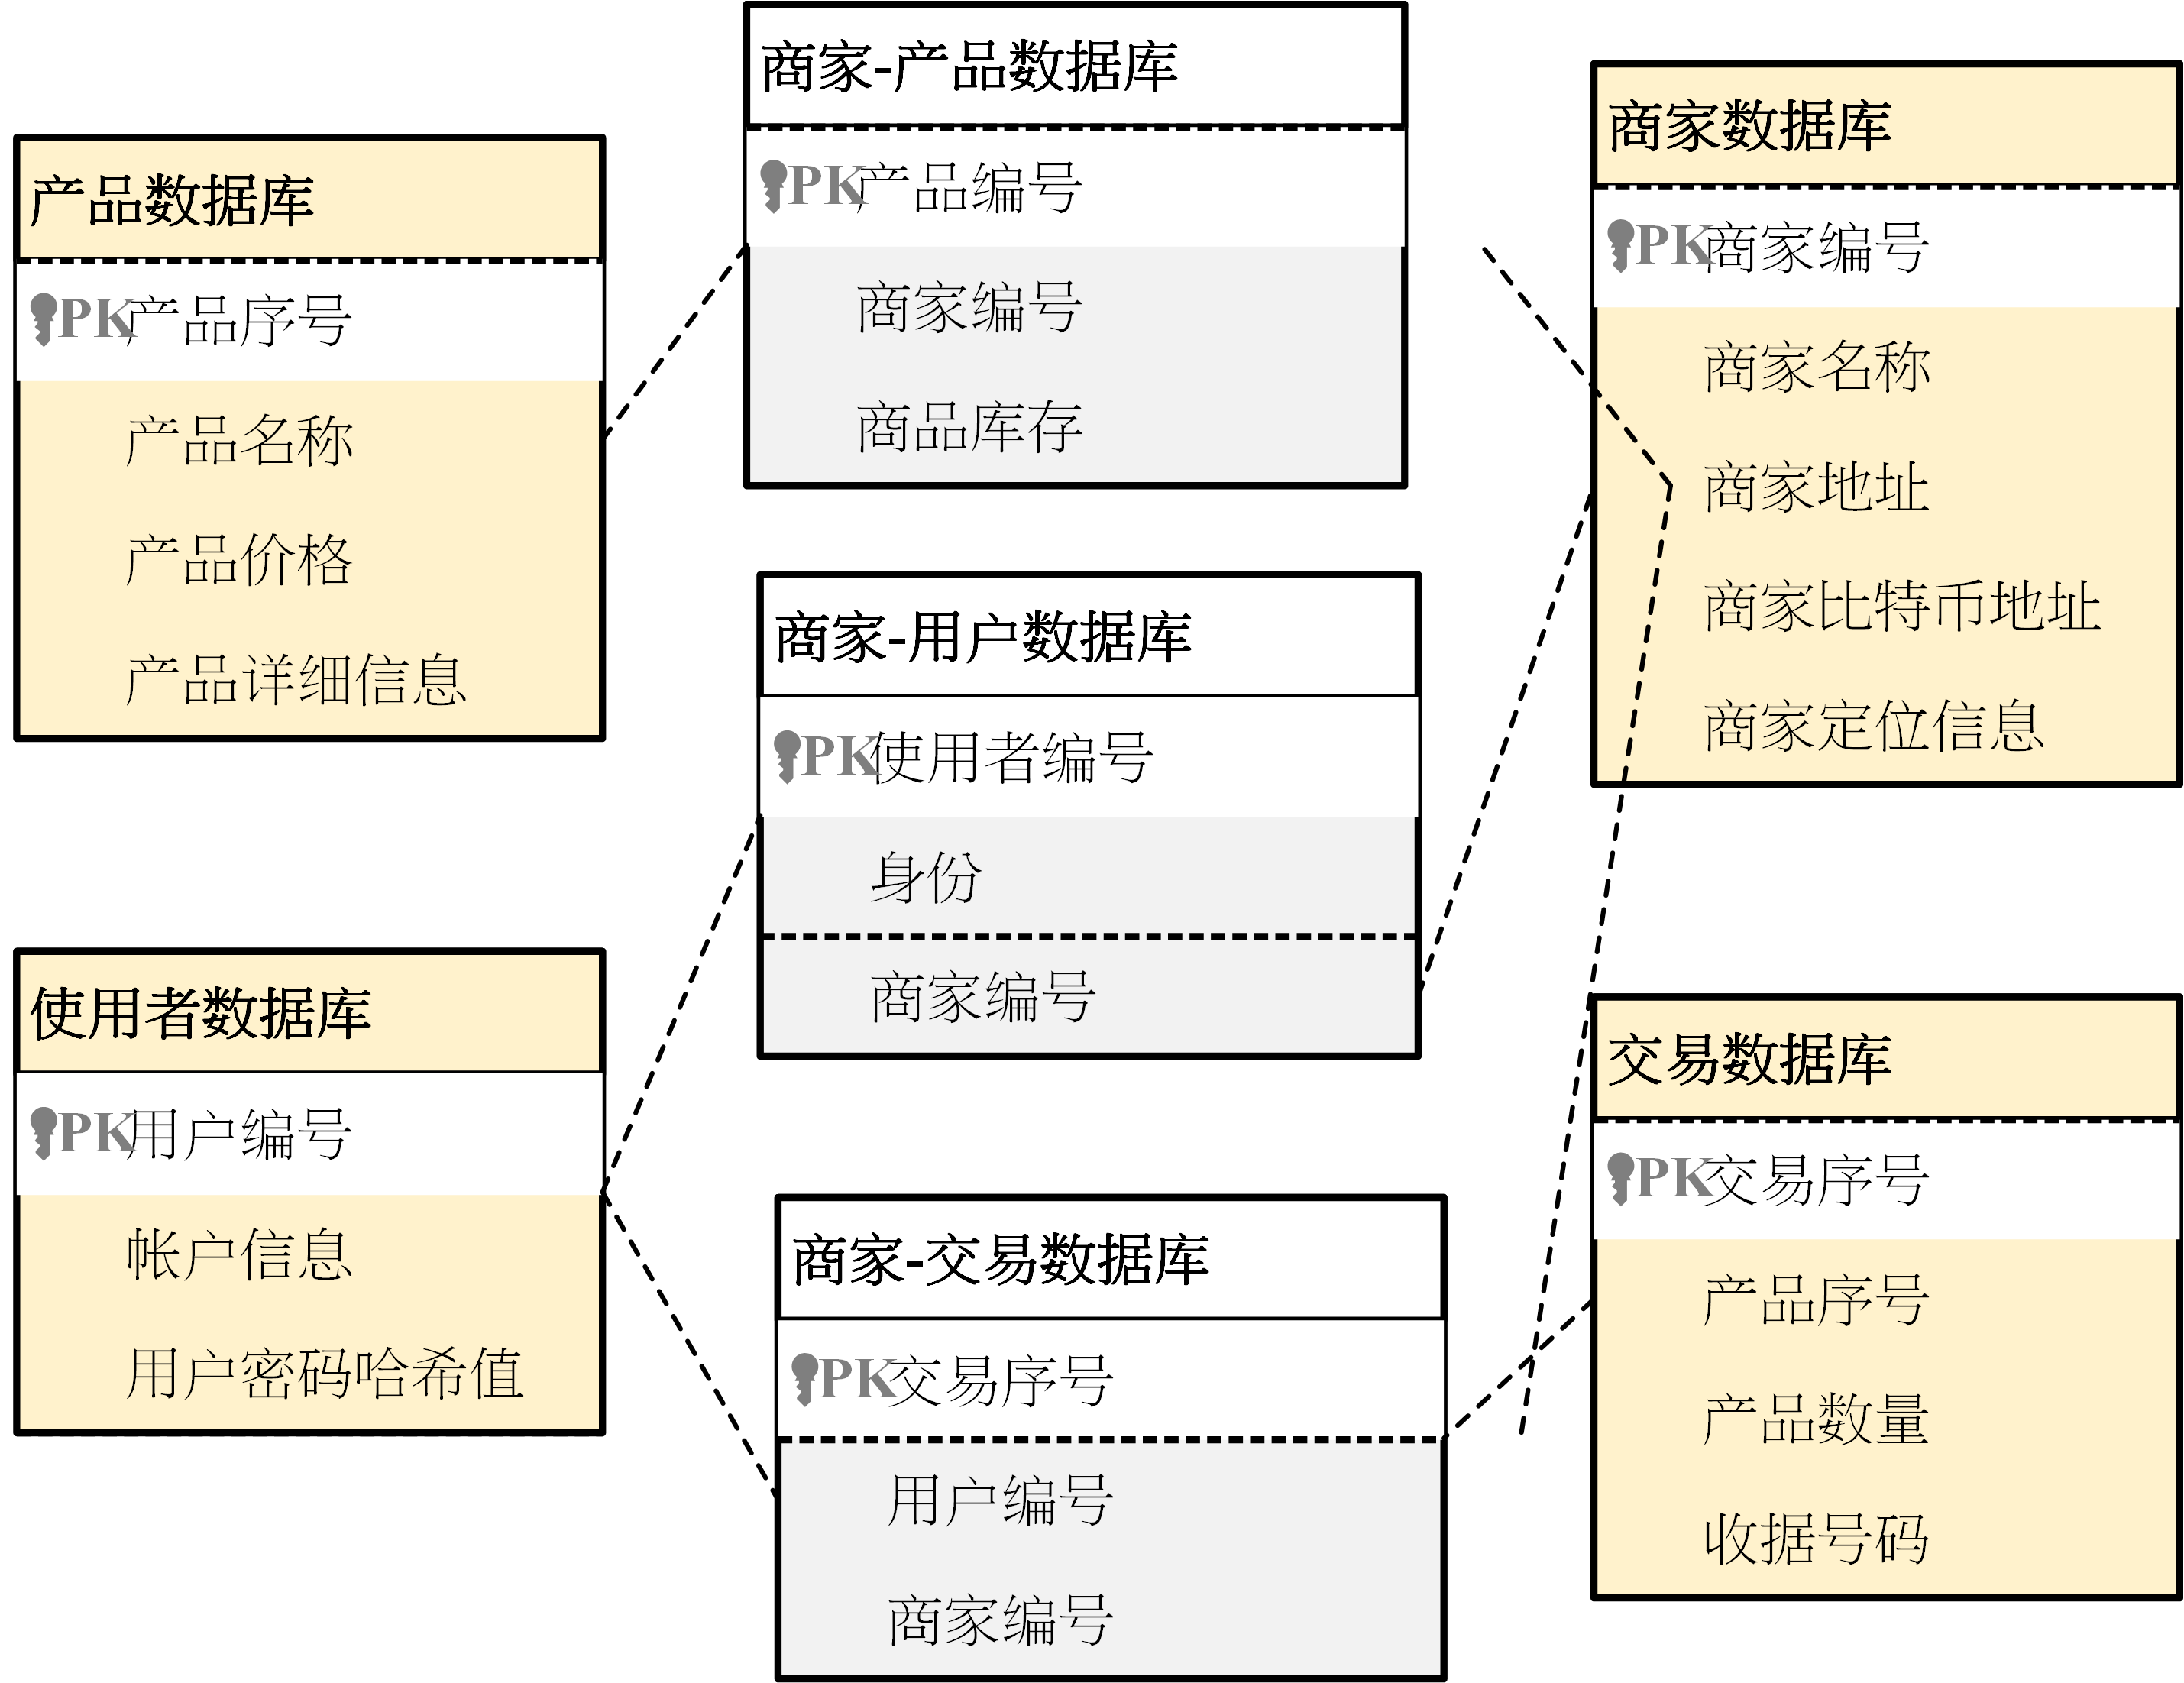
\includegraphics[width = 0.8\textwidth]{db.png}
			\caption{BRTMS數據庫分佈圖}\label{db}
		\end{figure}

			\paragraph{店家數據庫}存儲正在審核中的企業信息或已經過審核的企業信息。存儲的信息包括商家ID、商戶名稱、商戶位置、商戶的密碼貨幣地址以及GPS坐標。
			\paragraph{產品數據庫}只有授權用戶才能登錄添加或修改交易產品信息。產品數據庫內容包括產品標識號、產品名稱、產品說明、日期和價格等相關信息。
			\paragraph{交易數據庫}記錄包括交易序列號、產品識別號碼、產品交易金額、商戶密碼貨幣收款人地址、消費者密碼貨幣支付地址、商戶ID和最後確認字段的值。
			\paragraph{使用者數據庫}存儲所有使用者信息,包括政府、商家及顧客之個人帳戶信息的數據庫,而使用者密碼則以哈希的方式保存,以增加用戶安全性。

		\subsection{關聯數據庫}

			\paragraph{商家-用戶數據庫}本數據庫存儲各個商家擁有的職員信息,包括各店家的商店編號、使用者編號及身分編碼。
			\paragraph{商家-產品數據庫}此數據庫存儲各家公司當前商品存貨信息,由商店編號、產品編號及產品庫存所組成。
			\paragraph{商家-交易數據庫}本數據庫記錄著每一筆交易的經手人是誰,並由交易編號、店家序號,及使用者序號組成。

	\section{商店和商品信息管理子系統(SMIMSS)}
	在提出的区块链的实名交易监督系统架構中,商家需要在以下4個步驟中對商店和商品信息管理子系統(SMIMSS)進行註冊:

	\begin{figure}[h]
		\centering
		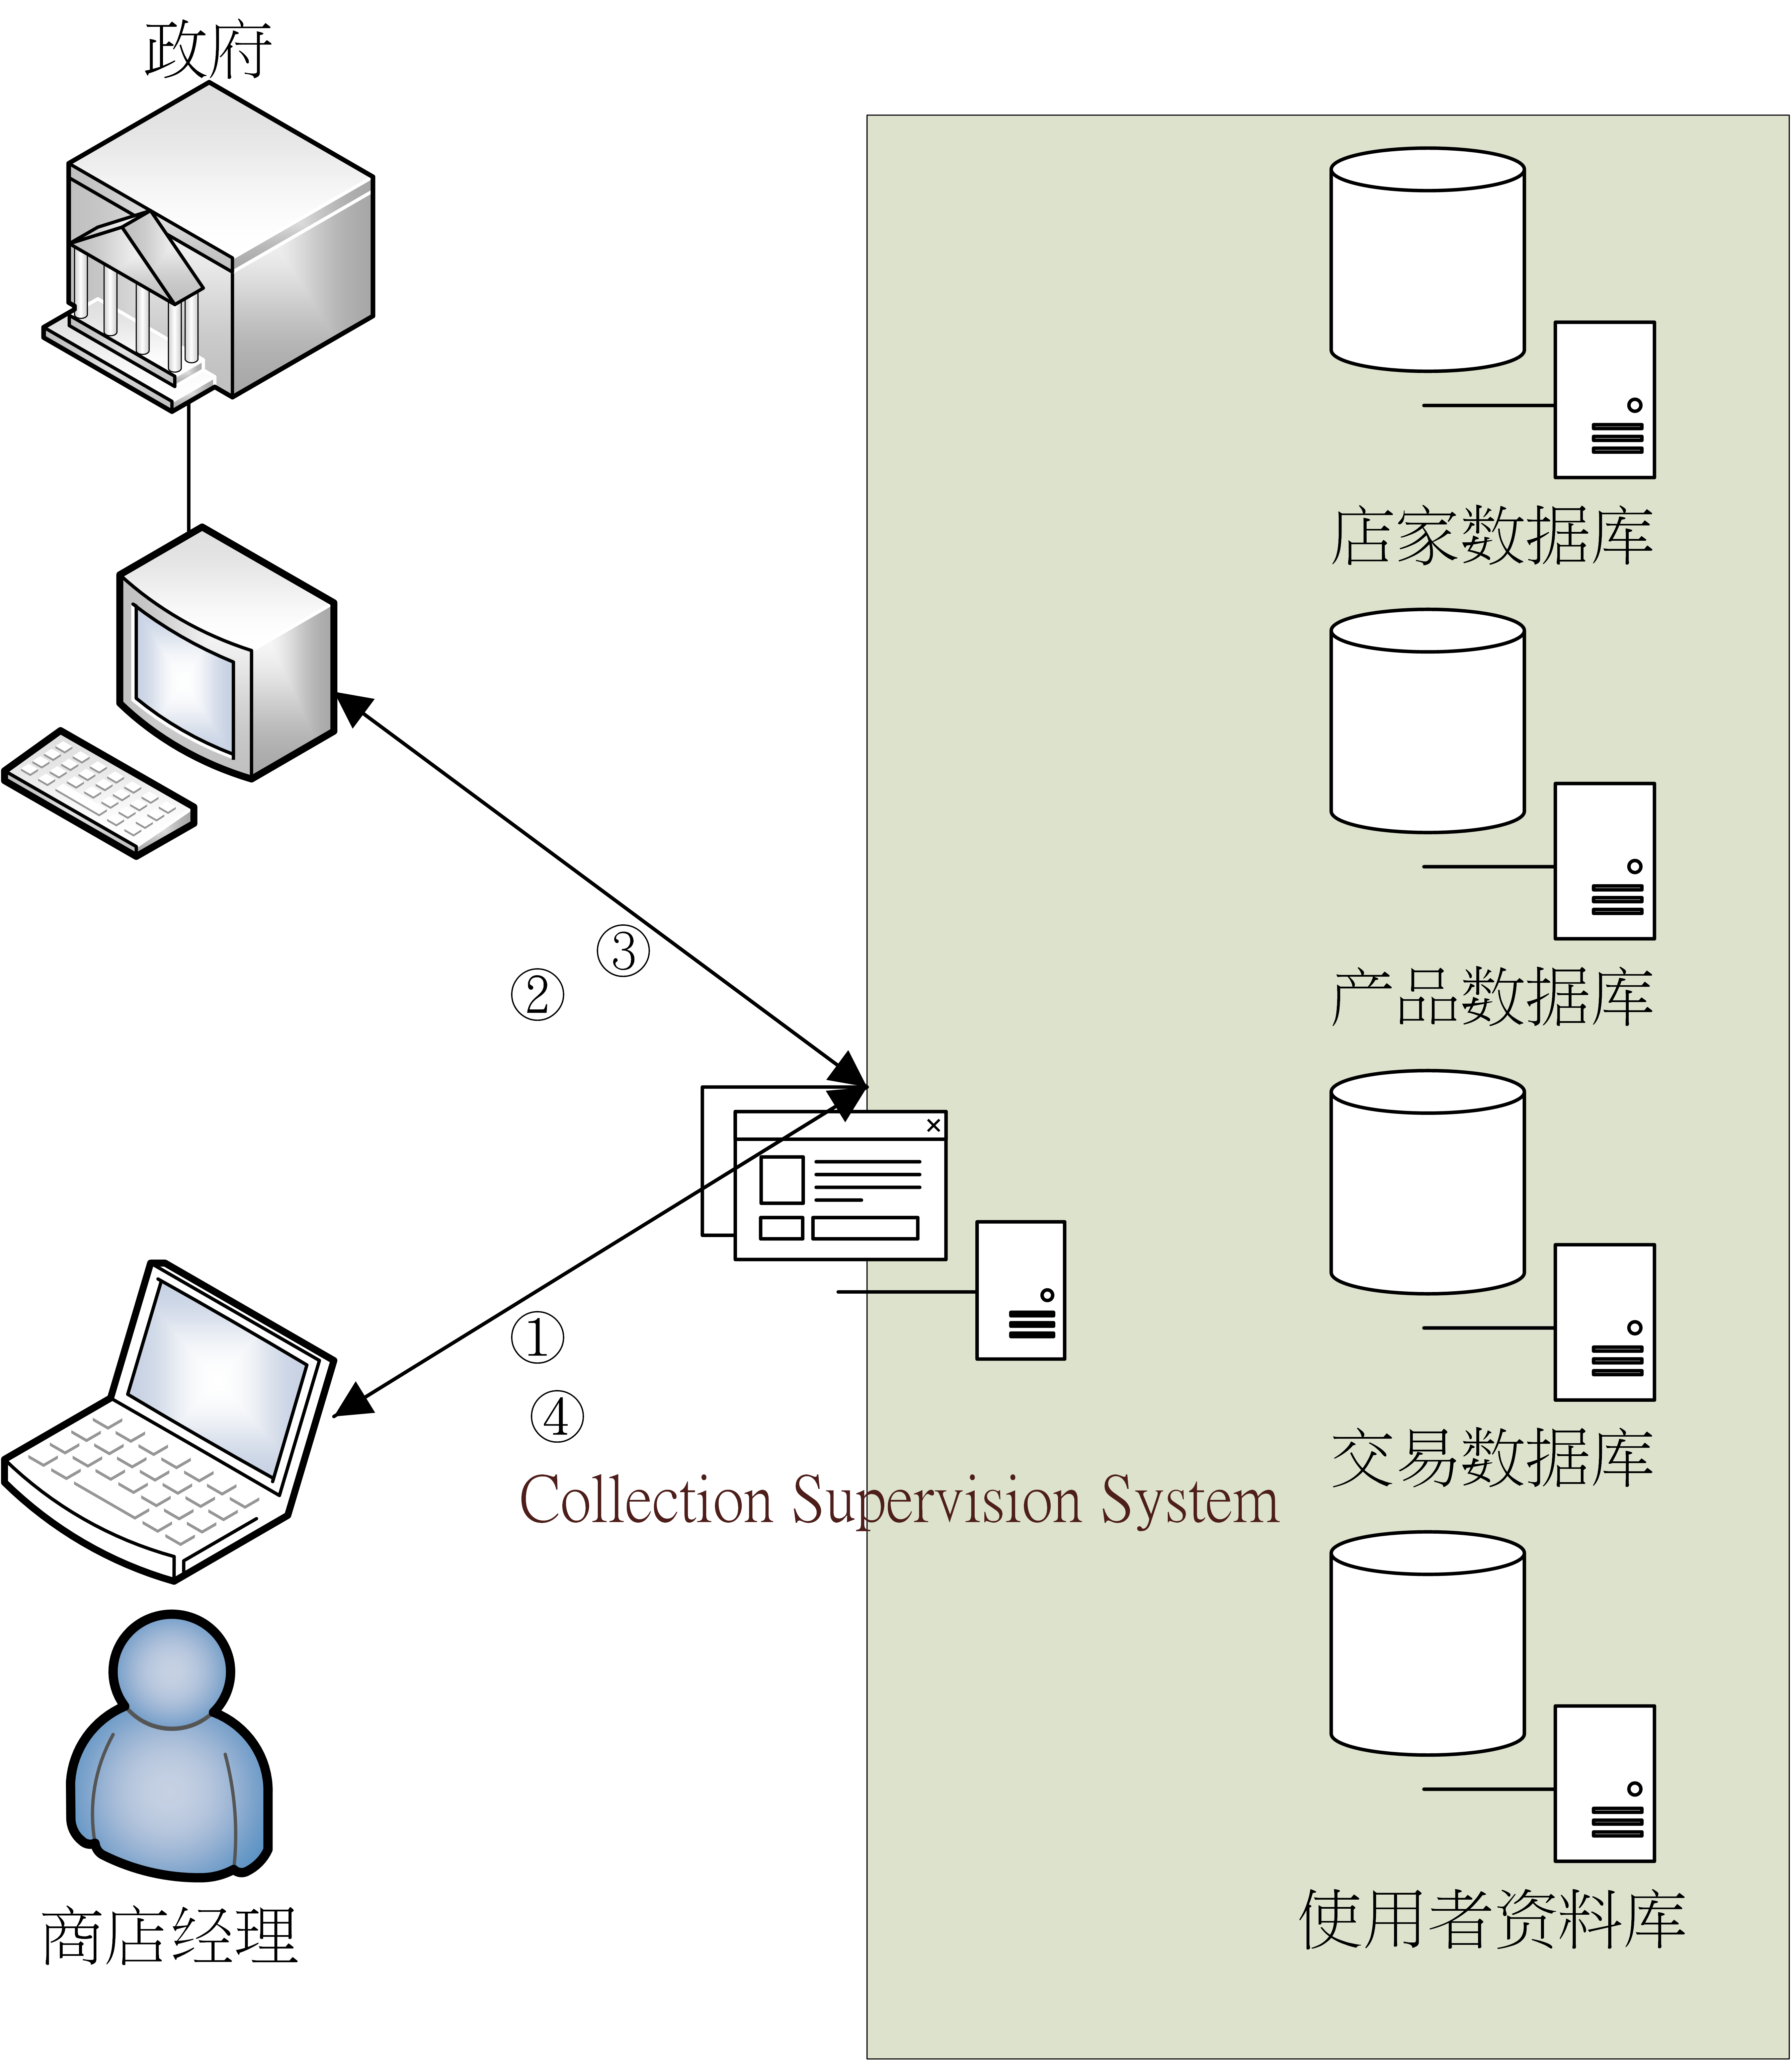
\includegraphics[width = 0.6\textwidth]{fig3.png}
		\caption{BRTMS和商家註冊流程的核心架構圖}\label{fig3}
	\end{figure}

	\begin{enumerate}
		\item 商戶必須在BRTMS註冊一個帳戶,並附有政府法規的商業證明。
		\item 区块链的实名交易监督系统將自動向相應的政府金融監管機構提交商業申請,以審查該商店的密碼貨幣交易業務。
		\item 如果政府批准商店的密碼貨幣業務申請,服務器將激活商家在該收集監控系統中創建商店帳戶。
		\item 商家可以自由地登錄賬戶並添加商家想要出售的產品,並檢查他們的密碼貨幣交易數據,例如產品庫存和產品交易記錄。
	\end{enumerate}

	\section{BRTMS架構與運作流程}
	具體的密碼貨幣商家收銀金流監控系統運行過程如圖\ref{fig4}所示,我們以圖\ref{fig3}所設計出的系統架構進行擴增,首先我們需要與blockchain explorer 對接,而之所以該監控系統需要與區塊鏈檢視器對接是為了能夠最直接的比對交易被記錄的成交狀況,能夠達到即時性以及正確性,倘若擔憂單方面的依賴相信區塊鏈檢視器的成果,亦可以使用多家區塊鏈檢視器進行交叉參考,以避免因為一家公司的錯誤所帶來的影響。區塊鏈檢視器的目的是為了能夠快速地準確地比對該筆交易的成交,做為整筆交易提出到結算的環節之一。

	\begin{figure}[h]
		\centering
		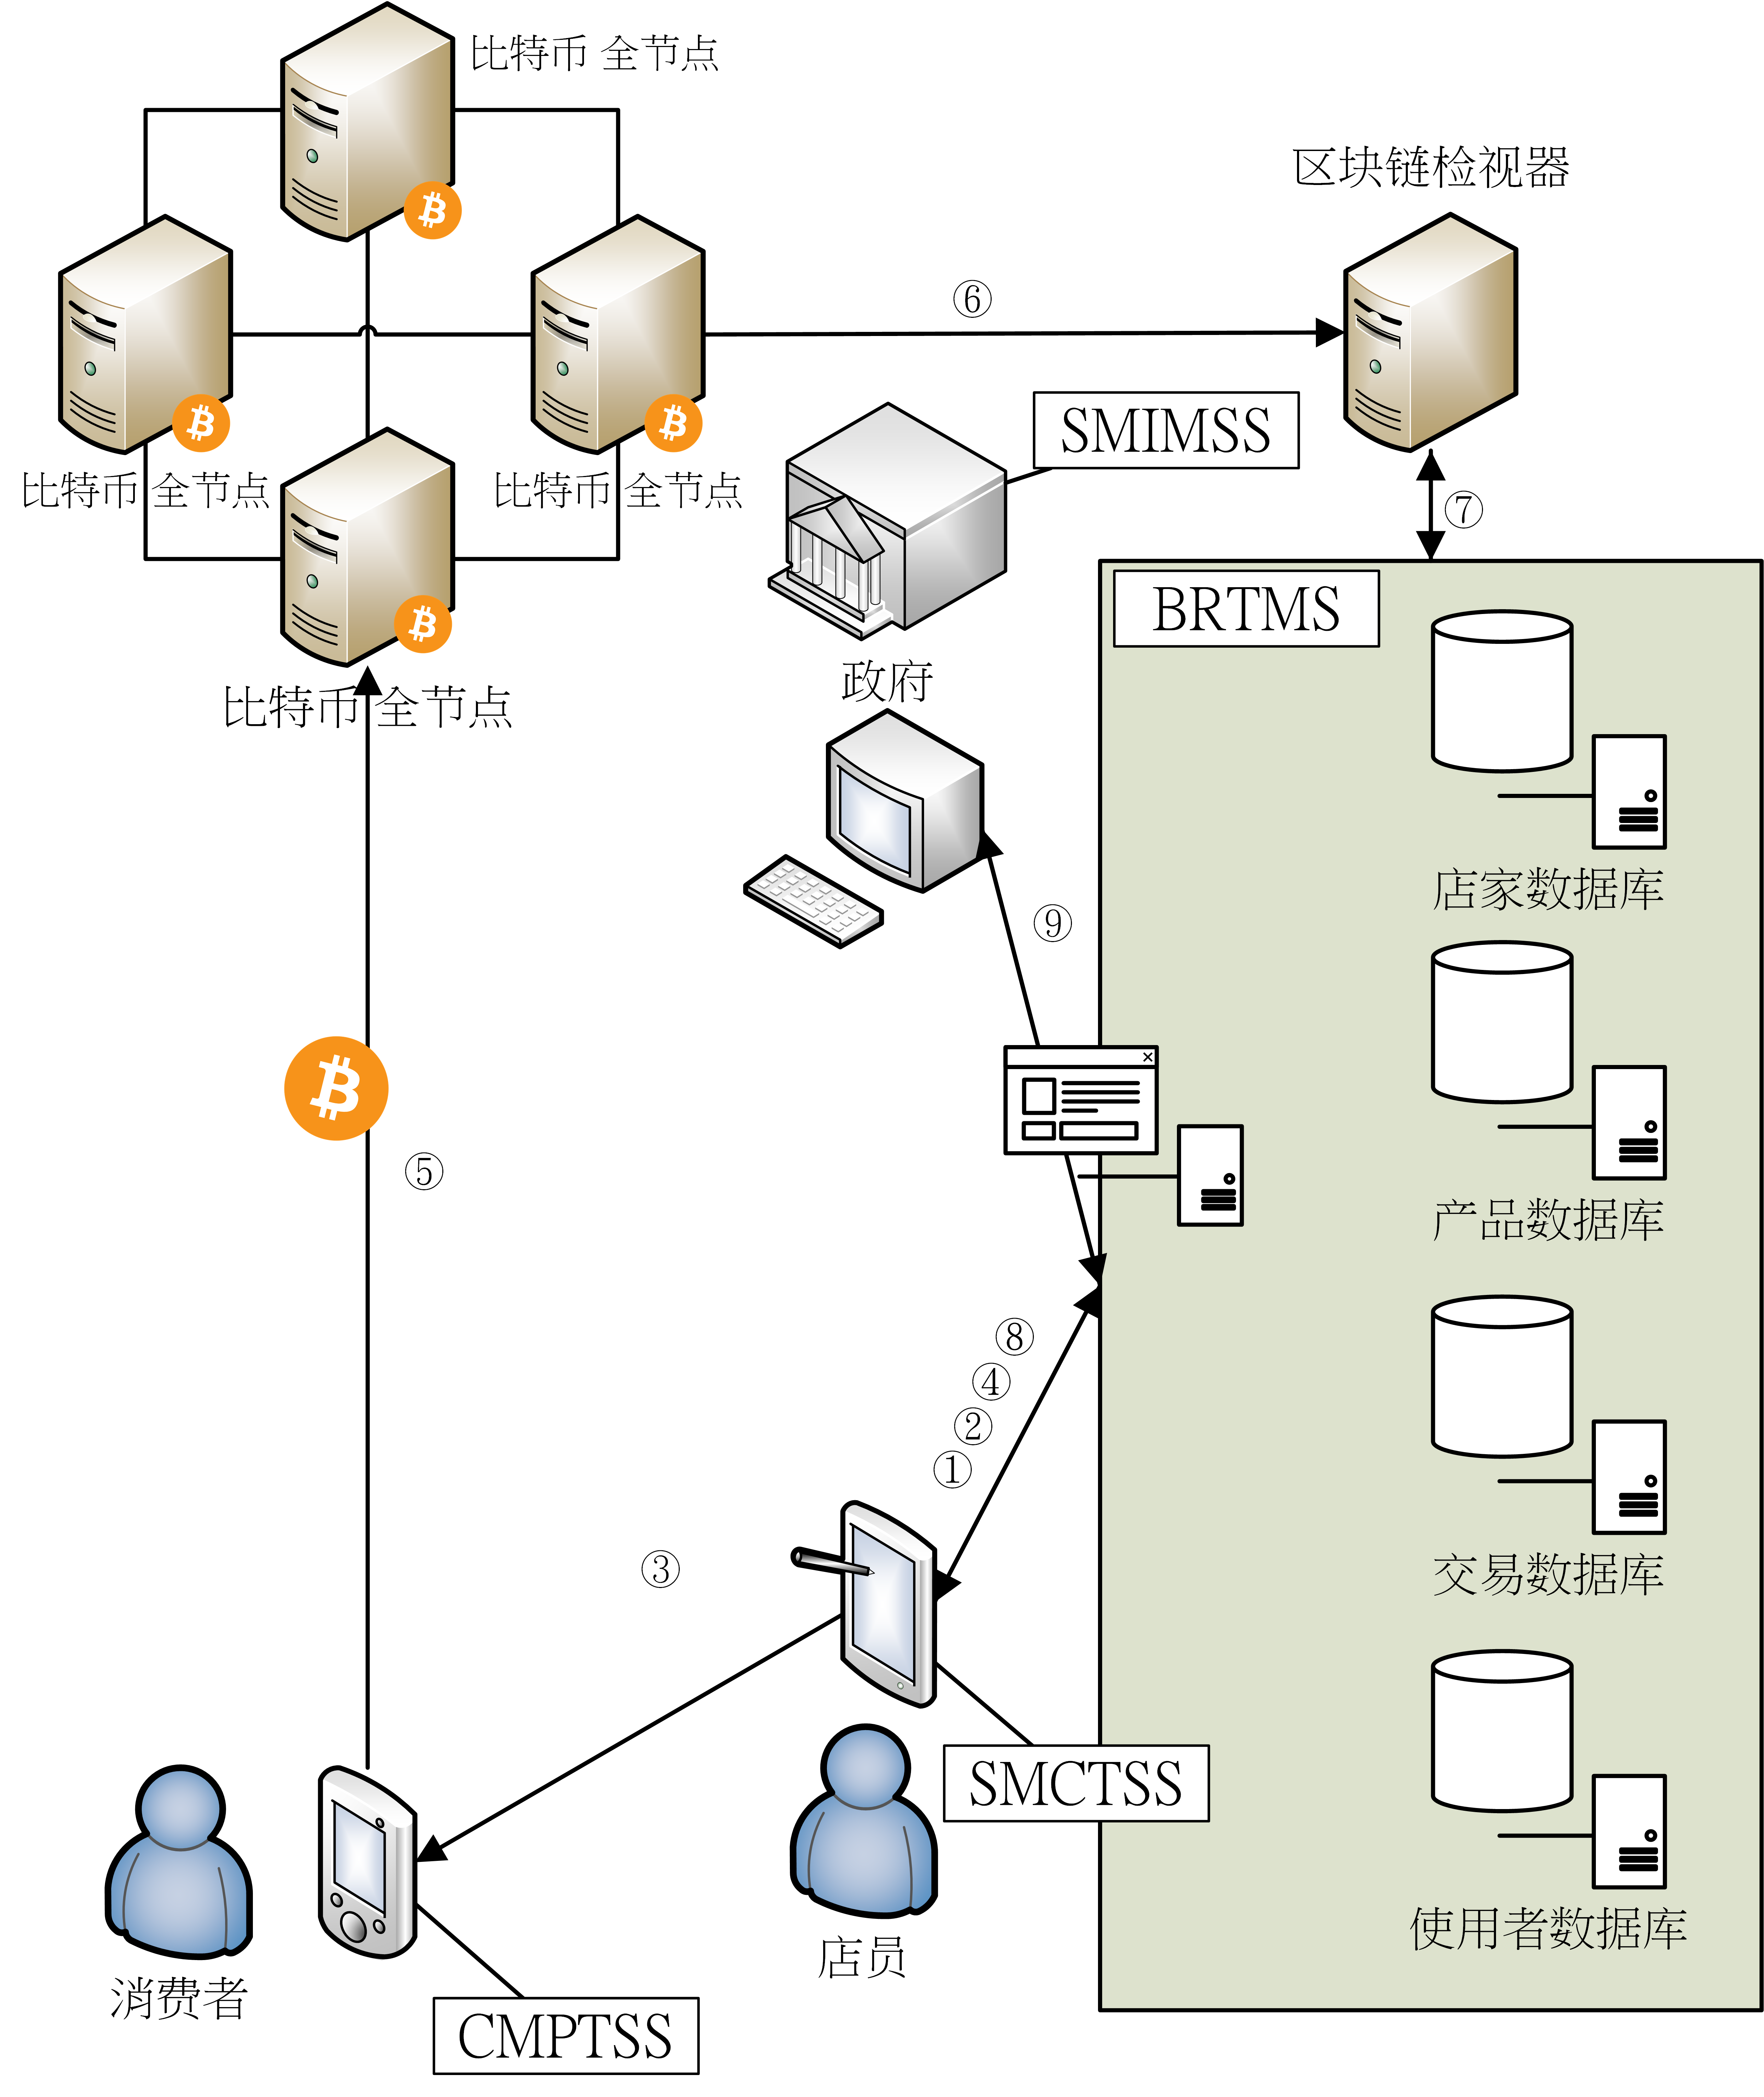
\includegraphics[width = 0.8\textwidth]{fig4.png}
		\caption{BRTMS的整體示意圖}\label{fig4}
	\end{figure}

	区块链的实名交易监督系统中創建步驟描述如下:

		\begin{enumerate}
			\item 商家的店員將登錄到如圖\ref{fig3}所示的先前步驟創建的帳戶,以使用手持式平板電腦或智能手機訪問SMCTSS中的服務。如前所述,在能夠登錄到系統之前,商家帳戶必須由政府機構審計。
			\item 在成功登錄SMCTSS用於商戶密碼貨幣流量監控系統時,移動設備將加載通過SMIMSS註冊的商店產品信息,然後創建產品目錄。商店的店員可以根據客戶的需求選擇所需的產品和數量。
			\item 店員使用設備完成客戶選定商品的產品信息後,移動設備上的NFC技術可用於將產品信息從附近店員的移動設備傳遞給消費者的移動設備,而無需物理交互。然後,消費者可以很容易地將自己的消費信息記錄成為發票等參考。在接收從商家店員設備向顧客設備購買產品消息的同時,顧客設備還將向商家的移動設備發送其自己的比特幣支付地址的消息。
			\item 商家的手持設備收到客戶確認購買所選產品的相應信息後,會將交易信息的副本發送給SMIMSS監控系統。消費者信息包括交易序列號、商戶ID號碼、商品號碼、購買的商品的數量以及密碼貨幣的收款人地址以及消費者的支付地址。
			\item 收到消費者交易信息後,即完成此次的密碼貨幣支付。同時,此次交易的密碼貨幣將發佈到比特幣網絡中進行驗證和記錄。
			\item 區塊鏈瀏覽器將開始分析在比特幣網絡中緩存的所有交易以及區塊鏈中記錄的交易。
			\item 擬議的交易監控系統BRTMS將向區塊鏈檢視器提出請求。這個請求數據不僅包括存儲在BRTMS中的交易副本之密碼貨幣收款人地址(如圖\ref{fig3}的第4步所述),還包括客戶預期付款的密碼貨幣支付地址。區塊鏈瀏覽器使用請求數據來檢查交易是否存儲在區塊鏈中,或者交易還在等待確認。如果交易已被確認並存儲在區塊鏈中,則交易數據庫中“交易確認”字段的值將更改為“1”,否則其默認值為"0"。
			\item 當“交易確認”字段中的值為“1”時,“交易已完成”消息可發送至商店平板電腦上運行的商店和商品信息管理子系統(SMCTSS)。
			\item 政府財政監督部門可以審查擬議BRTMS中的所有交易信息,以作為稅收審計參考。
		\end{enumerate}